\documentclass{beamer}
\usetheme{Berlin}
\usecolortheme{beaver}
\usepackage{graphicx}


\title{Modulation techniques}
\subtitle{Pulse amplitude modulation, Digital pulse modulation}
\author[Riccardo \and Eren]{Riccardo~Miccini\inst{1} \and Eren~Can~\inst{1}}
\institute[DTU]
{
	\inst{1}
	Technical University of Denmark\\
	Digital Communication
}
\date{\today}
\subject{Digital Communication}


\begin{document}

	\frame{\titlepage}

	\begin{frame}
		\frametitle{Analog Pulse Modulation techniques}
		\begin{itemize}
			\item Sample $ \rightarrow $ Pulse
			\item Pulse properties: amplitude, width, phase/position
			\item Modulation technique for each property: PAM, PWM, PPM
		\end{itemize}
	\end{frame}

	\begin{frame}
		\frametitle{Pulse Amplitude Modulation}
		\begin{itemize}
			\item Sequence of pulses with finite width $ \tau $
			\item Signal level $ \rightarrow $ pulse height
			\item Analog signal sampled at pulse edge: $ m_\delta = m(nT_s)\delta(t - nT_s) $
			\item Holding circuit: $ h(t) = rect(\frac{t - \frac{1}{2}\tau}{\tau}) $
		\end{itemize}
	\end{frame}

	\begin{frame}
		\frametitle{Delta Modulation}
		\begin{itemize}
			\item Delta modulation technique in which the message signal is encoded into a sequence of binary symbols.
			\item It is an analog to digital and digital to analog conversion technique.
			\item  It is the simplest form of DPCM cause the transmitted data are reduced to  a 1-bit
		\end{itemize}
	\end{frame}
<<<<<<< Updated upstream


=======
	
	\begin{frame}
	\frametitle{Explaining the functions and Figures}
	\begin{itemize}
	\item 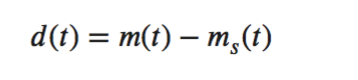
\includegraphics{Input for Pulse Modulator.png}
	\item 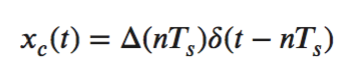
\includegraphics{Rewrtitten formula for dt.png}
    	\end{itemize}
         \end{frame}
         
         \begin{frame}
         \frametitle{Graphs for Delta Modulation}
         \includegraphics{
>>>>>>> Stashed changes
\end{document}
